% Requires in the preamble:
% \usepackage{amsmath,amssymb}
% \usepackage{tikz,pgfplots}
% \pgfplotsset{compat=1.18}

\chapter{Trigonometry in Radians}
\label{app:trigonometry-radians}

Trigonometry enters calculus whenever something turns, repeats, or oscillates.

A wheel rotates.  A spring vibrates.  A wave rises and falls.  A planet travels around
a focus.  A point on the unit circle moves with coordinates

\[
(\cos t,\sin t).
\]

That is why sine and cosine appear in derivatives, integrals, differential equations,
parametric curves, polar coordinates, complex numbers, and Fourier series.

This appendix reviews the trigonometry used in the book.  The main point is not to
memorize a long list of identities.  The main point is to know where the identities come
from: the unit circle, right triangles, and the Pythagorean Theorem.

One habit matters more than all the others:

\[
\boxed{
\text{In calculus, angles are measured in radians unless degrees are explicitly stated.}
}
\]

Radians make the formulas of calculus clean.

\section{Unit circle definitions}
\label{appsec:unit-circle-definitions}

Right triangles are a good beginning.  The unit circle is the calculus definition.

A right triangle defines sine and cosine only for acute angles.  But calculus needs
functions such as

\[
\sin x
\qquad\text{and}\qquad
\cos x
\]

for every real number \(x\).  The unit circle gives that definition.

\subsection{Radians and arc length}
\label{appsubsec:radians-arc-length}

A radian measures angle by arc length.

If a circle has radius \(r\), and a central angle \(\theta\) cuts off an arc of length \(s\),
then

\[
\boxed{
\theta=\frac{s}{r}
}
\]

when \(\theta\) is measured in radians.  Equivalently,

\[
\boxed{
s=r\theta.
}
\]

This formula is one of the reasons radians are the natural angle measure in calculus.
It says that angle is arc length divided by radius.

On the unit circle, where \(r=1\),

\[
s=\theta.
\]

So an angle of \(\theta\) radians is exactly an arc of length \(\theta\) on the unit circle.

\begin{figure}[h]
\centering
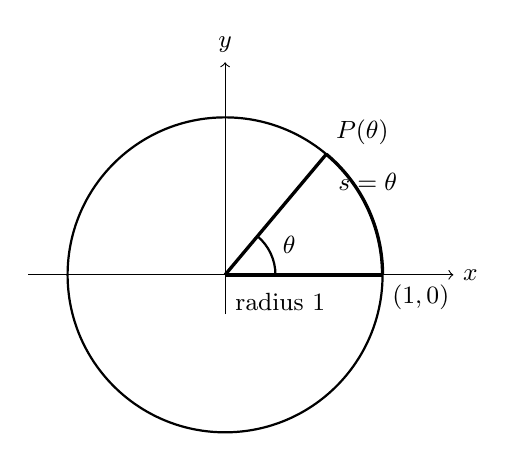
\begin{tikzpicture}[scale=2.0, every node/.style={font=\small}]
  \draw[->] (-1.25,0) -- (1.45,0) node[right] {\(x\)};
  \draw[->] (0,-0.25) -- (0,1.35) node[above] {\(y\)};

  \draw[thick] (0,0) circle (1);

  \def\ang{50}
  \coordinate (A) at (1,0);
  \coordinate (P) at ({cos(\ang)},{sin(\ang)});

  \draw[very thick] (0,0) -- (A);
  \draw[very thick] (0,0) -- (P);
  \draw[very thick] (A) arc (0:\ang:1);

  \draw[thick] (0.32,0) arc (0:\ang:0.32);
  \node at ({0.45*cos(25)},{0.45*sin(25)}) {\(\theta\)};

  \node[below right] at (A) {\((1,0)\)};
  \node[above right] at (P) {\(P(\theta)\)};
  \node[above] at ({cos(25)},{sin(25)+0.05}) {\(s=\theta\)};
  \node at (0.35,-0.17) {radius \(1\)};
\end{tikzpicture}
\caption{On the unit circle, radian measure equals arc length.}
\label{fig:appendix-unit-circle-arc}
\end{figure}

A full turn around a circle has circumference

\[
2\pi r.
\]

Dividing by \(r\), a full turn has angle

\[
2\pi
\]

radians.  Therefore

\[
\boxed{
2\pi\text{ radians}=360^\circ.
}
\]

So

\[
\boxed{
\pi\text{ radians}=180^\circ.
}
\]

To convert degrees to radians, multiply by

\[
\frac{\pi}{180}.
\]

To convert radians to degrees, multiply by

\[
\frac{180}{\pi}.
\]

\paragraph{Example.}
Convert \(150^\circ\) to radians.

\[
150^\circ
=
150\cdot\frac{\pi}{180}
=
\frac{5\pi}{6}.
\]

So

\[
\boxed{
150^\circ=\frac{5\pi}{6}\text{ radians}.
}
\]

\paragraph{Example.}
Convert \(\frac{7\pi}{4}\) radians to degrees.

\[
\frac{7\pi}{4}\cdot\frac{180}{\pi}
=
7\cdot45
=
315.
\]

So

\[
\boxed{
\frac{7\pi}{4}=315^\circ.
}
\]

\paragraph{Example.}
A circle has radius \(6\).  Find the arc length cut off by a central angle of
\(\frac{2\pi}{3}\) radians.

Use

\[
s=r\theta.
\]

Thus

\[
s=6\cdot\frac{2\pi}{3}=4\pi.
\]

So the arc length is

\[
\boxed{4\pi}.
\]

\subsection{Sine and cosine from the unit circle}
\label{appsubsec:sine-cosine-unit-circle}

Start at the point

\[
(1,0)
\]

on the unit circle.  Move counterclockwise along the circle through an arc of length
\(\theta\).  The point reached is called \(P(\theta)\).

If

\[
P(\theta)=(x,y),
\]

then we define

\[
\boxed{
\cos\theta=x
}
\]

and

\[
\boxed{
\sin\theta=y.
}
\]

So

\[
\boxed{
P(\theta)=(\cos\theta,\sin\theta).
}
\]

This definition works for every real number \(\theta\).  Positive \(\theta\) moves
counterclockwise.  Negative \(\theta\) moves clockwise.

\begin{figure}[h]
\centering
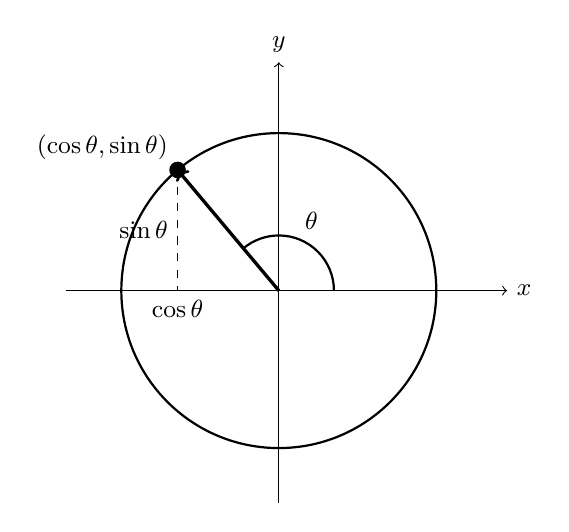
\begin{tikzpicture}[scale=2.0, every node/.style={font=\small}]
  \draw[->] (-1.35,0) -- (1.45,0) node[right] {\(x\)};
  \draw[->] (0,-1.35) -- (0,1.45) node[above] {\(y\)};

  \draw[thick] (0,0) circle (1);

  \def\ang{130}
  \coordinate (P) at ({cos(\ang)},{sin(\ang)});
  \coordinate (Q) at ({cos(\ang)},0);

  \draw[very thick,->] (0,0) -- (P);
  \draw[dashed] (P) -- (Q);
  \draw[dashed] (0,0) -- (Q);

  \draw[thick] (0.35,0) arc (0:\ang:0.35);
  \node at ({0.49*cos(65)},{0.49*sin(65)}) {\(\theta\)};

  \fill (P) circle (1.5pt);
  \node[above left] at (P) {\((\cos\theta,\sin\theta)\)};

  \node[below] at (Q) {\(\cos\theta\)};
  \node[left] at ({cos(\ang)}, {sin(\ang)/2}) {\(\sin\theta\)};
\end{tikzpicture}
\caption{The cosine is the \(x\)-coordinate and the sine is the \(y\)-coordinate on the unit circle.}
\label{fig:appendix-sine-cosine-coordinates}
\end{figure}

Because every point on the unit circle satisfies

\[
x^2+y^2=1,
\]

we immediately get

\[
\boxed{
\cos^2\theta+\sin^2\theta=1.
}
\]

This is the main identity of trigonometry.

\subsection{Tangent, secant, cosecant, and cotangent}
\label{appsubsec:other-trig-functions}

The other trigonometric functions are built from sine and cosine.

\[
\boxed{
\tan\theta=\frac{\sin\theta}{\cos\theta}
}
\qquad
\text{when }\cos\theta\neq0.
\]

\[
\boxed{
\sec\theta=\frac1{\cos\theta}
}
\qquad
\text{when }\cos\theta\neq0.
\]

\[
\boxed{
\csc\theta=\frac1{\sin\theta}
}
\qquad
\text{when }\sin\theta\neq0.
\]

\[
\boxed{
\cot\theta=\frac{\cos\theta}{\sin\theta}
}
\qquad
\text{when }\sin\theta\neq0.
\]

The restrictions matter.  Division by zero is still forbidden.

For example,

\[
\cos\left(\frac{\pi}{2}\right)=0,
\]

so

\[
\tan\left(\frac{\pi}{2}\right)
\]

and

\[
\sec\left(\frac{\pi}{2}\right)
\]

are undefined.

\subsection{Special angles}
\label{appsubsec:special-angles}

The most common exact values come from the \(30^\circ\)-\(60^\circ\)-\(90^\circ\)
triangle and the \(45^\circ\)-\(45^\circ\)-\(90^\circ\) triangle.

In radians, these angles are

\[
\frac{\pi}{6},
\qquad
\frac{\pi}{3},
\qquad
\frac{\pi}{4}.
\]

\begin{center}
\renewcommand{\arraystretch}{1.7}
\begin{tabular}{c|ccccc}
\(\theta\) & \(0\) & \(\dfrac{\pi}{6}\) & \(\dfrac{\pi}{4}\) &
\(\dfrac{\pi}{3}\) & \(\dfrac{\pi}{2}\) \\ \hline
\(\sin\theta\) & \(0\) & \(\dfrac12\) & \(\dfrac{\sqrt2}{2}\) &
\(\dfrac{\sqrt3}{2}\) & \(1\) \\[6pt]
\(\cos\theta\) & \(1\) & \(\dfrac{\sqrt3}{2}\) & \(\dfrac{\sqrt2}{2}\) &
\(\dfrac12\) & \(0\) \\[6pt]
\(\tan\theta\) & \(0\) & \(\dfrac{\sqrt3}{3}\) & \(1\) &
\(\sqrt3\) & \text{undefined}
\end{tabular}
\end{center}

These first-quadrant values, together with signs and symmetry, give the exact values
in the other quadrants.

\begin{center}
\renewcommand{\arraystretch}{1.5}
\begin{tabular}{c|ccc}
\textbf{quadrant} & \(\sin\theta\) & \(\cos\theta\) & \(\tan\theta\) \\ \hline
I & \(+\) & \(+\) & \(+\) \\
II & \(+\) & \(-\) & \(-\) \\
III & \(-\) & \(-\) & \(+\) \\
IV & \(-\) & \(+\) & \(-\)
\end{tabular}
\end{center}

\paragraph{Example.}
Find

\[
\sin\left(\frac{5\pi}{6}\right),
\qquad
\cos\left(\frac{5\pi}{6}\right),
\qquad
\tan\left(\frac{5\pi}{6}\right).
\]

The angle

\[
\frac{5\pi}{6}
\]

lies in Quadrant II.  Its reference angle is

\[
\pi-\frac{5\pi}{6}=\frac{\pi}{6}.
\]

In Quadrant II, sine is positive and cosine is negative.  Therefore

\[
\sin\left(\frac{5\pi}{6}\right)=\frac12,
\]

\[
\cos\left(\frac{5\pi}{6}\right)=-\frac{\sqrt3}{2},
\]

and

\[
\tan\left(\frac{5\pi}{6}\right)
=
\frac{\sin(5\pi/6)}{\cos(5\pi/6)}
=
-\frac1{\sqrt3}
=
-\frac{\sqrt3}{3}.
\]

\subsection{Periodicity and coterminal angles}
\label{appsubsec:periodicity-coterminal}

Adding \(2\pi\) radians makes one full turn around the unit circle.  The point on the
circle does not change.  Therefore

\[
\boxed{
\sin(\theta+2\pi)=\sin\theta
}
\]

and

\[
\boxed{
\cos(\theta+2\pi)=\cos\theta.
}
\]

For any integer \(k\),

\[
\boxed{
\sin(\theta+2\pi k)=\sin\theta,
\qquad
\cos(\theta+2\pi k)=\cos\theta.
}
\]

Angles that differ by a multiple of \(2\pi\) are called \emph{coterminal angles}.

Tangent has period \(\pi\), because opposite points on the unit circle have both sine
and cosine signs reversed, so the quotient is unchanged:

\[
\boxed{
\tan(\theta+\pi)=\tan\theta.
}
\]

\paragraph{Example.}
Find

\[
\cos\left(\frac{17\pi}{6}\right).
\]

Subtract \(2\pi=\frac{12\pi}{6}\):

\[
\frac{17\pi}{6}-2\pi
=
\frac{17\pi}{6}-\frac{12\pi}{6}
=
\frac{5\pi}{6}.
\]

So

\[
\cos\left(\frac{17\pi}{6}\right)
=
\cos\left(\frac{5\pi}{6}\right)
=
-\frac{\sqrt3}{2}.
\]

\subsection{Graphs of sine and cosine}
\label{appsubsec:graphs-sine-cosine-review}

The unit circle produces the graphs of sine and cosine as the angle changes.

Both functions have period \(2\pi\).  The sine graph starts at \(0\), rises to \(1\), returns
to \(0\), falls to \(-1\), and returns to \(0\).

The cosine graph starts at \(1\), falls to \(0\), reaches \(-1\), returns to \(0\), and
then returns to \(1\).

\begin{figure}[h]
\centering
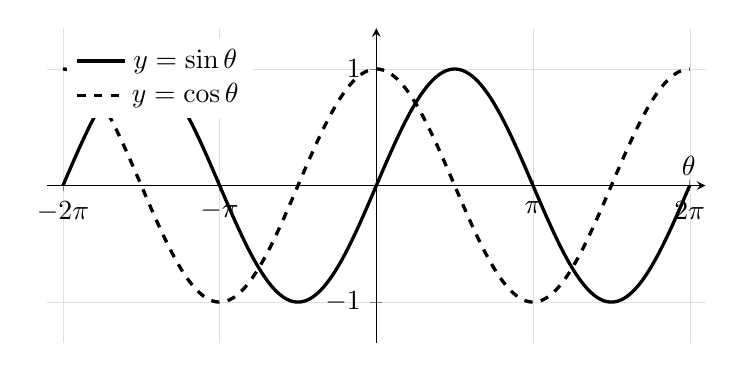
\begin{tikzpicture}
\begin{axis}[
    width=0.82\textwidth,
    height=0.46\textwidth,
    xmin=-6.6, xmax=6.6,
    ymin=-1.35, ymax=1.35,
    axis lines=middle,
    xlabel={\(\theta\)},
    ylabel={},
    xtick={-6.283,-3.142,0,3.142,6.283},
    xticklabels={\(-2\pi\),\(-\pi\),\(0\),\(\pi\),\(2\pi\)},
    ytick={-1,0,1},
    grid=both,
    grid style={line width=.1pt, draw=gray!25},
    legend style={draw=none, at={(0.03,0.97)}, anchor=north west}
]
\addplot[very thick, domain=-6.283:6.283, samples=250] {sin(deg(x))};
\addlegendentry{\(y=\sin\theta\)}
\addplot[very thick, dashed, domain=-6.283:6.283, samples=250] {cos(deg(x))};
\addlegendentry{\(y=\cos\theta\)}
\end{axis}
\end{tikzpicture}
\caption{Sine and cosine are periodic because the unit circle repeats after a full turn.}
\label{fig:appendix-sine-cosine-graphs}
\end{figure}

These graphs are not only pictures.  Later, their slopes give

\[
(\sin x)'=\cos x
\]

and

\[
(\cos x)'=-\sin x.
\]

Those formulas are this circular motion translated into calculus.

\section{Basic identities}
\label{appsec:basic-trig-identities}

Trigonometric identities are equations that are true for every angle where both sides
are defined.

They are useful because they let us change the form of an expression without changing
its value.  In calculus, this can turn a difficult derivative or integral into an easier one.

\subsection{Reciprocal and quotient identities}
\label{appsubsec:reciprocal-quotient-identities}

The reciprocal identities come directly from the definitions:

\[
\boxed{
\sec x=\frac1{\cos x},
\qquad
\csc x=\frac1{\sin x},
\qquad
\cot x=\frac1{\tan x}.
}
\]

The quotient identities are

\[
\boxed{
\tan x=\frac{\sin x}{\cos x},
\qquad
\cot x=\frac{\cos x}{\sin x}.
}
\]

Each identity is valid only where the denominators are nonzero.

\paragraph{Example.}
Simplify

\[
\sin x\sec x.
\]

Since

\[
\sec x=\frac1{\cos x},
\]

we get

\[
\sin x\sec x
=
\sin x\cdot\frac1{\cos x}
=
\frac{\sin x}{\cos x}.
\]

Therefore

\[
\boxed{
\sin x\sec x=\tan x
}
\]

where \(\cos x\neq0\).

\subsection{Pythagorean identities}
\label{appsubsec:pythagorean-identities}

The main identity comes from the unit circle:

\[
\boxed{
\sin^2 x+\cos^2 x=1.
}
\]

Here

\[
\sin^2 x
\]

means

\[
(\sin x)^2,
\]

not

\[
\sin(x^2).
\]

Dividing

\[
\sin^2 x+\cos^2 x=1
\]

by \(\cos^2 x\), where \(\cos x\neq0\), gives

\[
\tan^2 x+1=\sec^2 x.
\]

So

\[
\boxed{
1+\tan^2 x=\sec^2 x.
}
\]

Dividing by \(\sin^2 x\), where \(\sin x\neq0\), gives

\[
1+\cot^2 x=\csc^2 x.
\]

Thus

\[
\boxed{
1+\cot^2 x=\csc^2 x.
}
\]

\begin{center}
\renewcommand{\arraystretch}{1.7}
\begin{tabular}{c}
\textbf{Pythagorean identities} \\ \hline
\(\sin^2 x+\cos^2 x=1\) \\[3pt]
\(1+\tan^2 x=\sec^2 x\) \\[3pt]
\(1+\cot^2 x=\csc^2 x\)
\end{tabular}
\end{center}

\paragraph{Example.}
Simplify

\[
1-\cos^2 x.
\]

From

\[
\sin^2 x+\cos^2 x=1,
\]

we get

\[
1-\cos^2 x=\sin^2 x.
\]

So

\[
\boxed{
1-\cos^2 x=\sin^2 x.
}
\]

\paragraph{Example.}
Simplify

\[
\sec^2 x-\tan^2 x.
\]

Using

\[
1+\tan^2 x=\sec^2 x,
\]

we get

\[
\sec^2 x-\tan^2 x=1.
\]

Thus

\[
\boxed{
\sec^2 x-\tan^2 x=1.
}
\]

\subsection{Even and odd identities}
\label{appsubsec:even-odd-trig-identities}

On the unit circle, replacing \(x\) by \(-x\) reflects the point across the \(x\)-axis.
The \(x\)-coordinate stays the same, while the \(y\)-coordinate changes sign.

Therefore

\[
\boxed{
\cos(-x)=\cos x
}
\]

and

\[
\boxed{
\sin(-x)=-\sin x.
}
\]

Since

\[
\tan x=\frac{\sin x}{\cos x},
\]

we also have

\[
\boxed{
\tan(-x)=-\tan x.
}
\]

So cosine is even, while sine and tangent are odd.

\begin{center}
\renewcommand{\arraystretch}{1.5}
\begin{tabular}{c|c}
\textbf{identity} & \textbf{meaning} \\ \hline
\(\cos(-x)=\cos x\) & cosine is even \\
\(\sin(-x)=-\sin x\) & sine is odd \\
\(\tan(-x)=-\tan x\) & tangent is odd
\end{tabular}
\end{center}

\paragraph{Example.}
Simplify

\[
\sin(-x)\cos(-x).
\]

Use the even and odd identities:

\[
\sin(-x)\cos(-x)
=
(-\sin x)(\cos x).
\]

Therefore

\[
\boxed{
\sin(-x)\cos(-x)=-\sin x\cos x.
}
\]

\subsection{Using identities carefully}
\label{appsubsec:using-identities-carefully}

Trigonometric identities can simplify expressions, but they must be used with the same
care as algebraic identities.

\begin{quote}
\textbf{Warning.}
Never divide by a trigonometric expression unless you know it is not zero.

For example, the equation

\[
\sin x\cos x=\sin x
\]

cannot be simplified by blindly dividing by \(\sin x\).  Some solutions may have
\(\sin x=0\).
\end{quote}

\paragraph{Example.}
Solve

\[
\sin x\cos x=\sin x
\]

on

\[
0\le x<2\pi.
\]

Move all terms to one side:

\[
\sin x\cos x-\sin x=0.
\]

Factor:

\[
\sin x(\cos x-1)=0.
\]

Thus

\[
\sin x=0
\qquad\text{or}\qquad
\cos x-1=0.
\]

On \(0\le x<2\pi\),

\[
\sin x=0
\]

at

\[
x=0,\ \pi.
\]

Also,

\[
\cos x=1
\]

at

\[
x=0.
\]

So the solutions are

\[
\boxed{
x=0,\ \pi.
}
\]

If we had divided by \(\sin x\), we would have lost the solution \(x=\pi\).

\section{Addition formulas}
\label{appsec:addition-formulas}

The basic identities came from one angle.  The addition formulas tell how two angles
combine.

They are the source of many identities used in differentiation and integration.

\subsection{Cosine of a difference}
\label{appsubsec:cosine-difference}

Take two points on the unit circle:

\[
P=(\cos a,\sin a),
\qquad
Q=(\cos b,\sin b).
\]

The distance between these two points depends only on the angle between them, which is
\(a-b\).

Using the distance formula,

\[
\text{distance}^2
=
(\cos a-\cos b)^2+(\sin a-\sin b)^2.
\]

Expand:

\[
\text{distance}^2
=
\cos^2 a-2\cos a\cos b+\cos^2 b
+
\sin^2 a-2\sin a\sin b+\sin^2 b.
\]

Group terms:

\[
\text{distance}^2
=
(\cos^2 a+\sin^2 a)
+
(\cos^2 b+\sin^2 b)
-
2(\cos a\cos b+\sin a\sin b).
\]

Since each point is on the unit circle,

\[
\cos^2 a+\sin^2 a=1,
\qquad
\cos^2 b+\sin^2 b=1.
\]

Thus

\[
\text{distance}^2
=
2-2(\cos a\cos b+\sin a\sin b).
\]

On the other hand, the same distance is the distance from \((1,0)\) to the point
at angle \(a-b\).  That squared distance is

\[
(\cos(a-b)-1)^2+\sin^2(a-b).
\]

Expand:

\[
\cos^2(a-b)-2\cos(a-b)+1+\sin^2(a-b).
\]

Using

\[
\cos^2(a-b)+\sin^2(a-b)=1,
\]

this becomes

\[
2-2\cos(a-b).
\]

The two squared distances are equal, so

\[
2-2\cos(a-b)
=
2-2(\cos a\cos b+\sin a\sin b).
\]

Therefore

\[
\boxed{
\cos(a-b)=\cos a\cos b+\sin a\sin b.
}
\]

This identity is the anchor.  The other addition formulas follow from it.

\subsection{Sine and cosine addition formulas}
\label{appsubsec:sine-cosine-addition}

The addition formulas are:

\[
\boxed{
\sin(a+b)=\sin a\cos b+\cos a\sin b
}
\]

\[
\boxed{
\sin(a-b)=\sin a\cos b-\cos a\sin b
}
\]

\[
\boxed{
\cos(a+b)=\cos a\cos b-\sin a\sin b
}
\]

\[
\boxed{
\cos(a-b)=\cos a\cos b+\sin a\sin b.
}
\]

A common mistake is to distribute sine or cosine over addition.  That is not correct:

\[
\sin(a+b)\neq \sin a+\sin b,
\]

and

\[
\cos(a+b)\neq \cos a+\cos b.
\]

For example,

\[
\sin\left(\frac{\pi}{2}\right)=1,
\]

but

\[
\sin\left(\frac{\pi}{4}\right)+\sin\left(\frac{\pi}{4}\right)
=
\frac{\sqrt2}{2}+\frac{\sqrt2}{2}
=
\sqrt2.
\]

So

\[
\sin\left(\frac{\pi}{4}+\frac{\pi}{4}\right)
\neq
\sin\left(\frac{\pi}{4}\right)+\sin\left(\frac{\pi}{4}\right).
\]

\paragraph{Example.}
Find the exact value of

\[
\sin\left(\frac{5\pi}{12}\right).
\]

Notice that

\[
\frac{5\pi}{12}
=
\frac{\pi}{4}+\frac{\pi}{6}.
\]

Using the sine addition formula,

\[
\sin\left(\frac{\pi}{4}+\frac{\pi}{6}\right)
=
\sin\frac{\pi}{4}\cos\frac{\pi}{6}
+
\cos\frac{\pi}{4}\sin\frac{\pi}{6}.
\]

Substitute exact values:

\[
=
\frac{\sqrt2}{2}\cdot\frac{\sqrt3}{2}
+
\frac{\sqrt2}{2}\cdot\frac12.
\]

Thus

\[
\boxed{
\sin\left(\frac{5\pi}{12}\right)
=
\frac{\sqrt6+\sqrt2}{4}.
}
\]

\paragraph{Example.}
Simplify

\[
\cos\left(x-\frac{\pi}{2}\right).
\]

Use

\[
\cos(a-b)=\cos a\cos b+\sin a\sin b.
\]

Then

\[
\cos\left(x-\frac{\pi}{2}\right)
=
\cos x\cos\frac{\pi}{2}
+
\sin x\sin\frac{\pi}{2}.
\]

Since

\[
\cos\frac{\pi}{2}=0,
\qquad
\sin\frac{\pi}{2}=1,
\]

we get

\[
\boxed{
\cos\left(x-\frac{\pi}{2}\right)=\sin x.
}
\]

\subsection{Tangent addition formulas}
\label{appsubsec:tangent-addition}

Because

\[
\tan x=\frac{\sin x}{\cos x},
\]

the tangent formulas follow from the sine and cosine formulas.

\[
\boxed{
\tan(a+b)=\frac{\tan a+\tan b}{1-\tan a\tan b}
}
\]

and

\[
\boxed{
\tan(a-b)=\frac{\tan a-\tan b}{1+\tan a\tan b}.
}
\]

These formulas are valid where the expressions involved are defined.

\paragraph{Example.}
Find

\[
\tan\left(\frac{7\pi}{12}\right).
\]

Write

\[
\frac{7\pi}{12}
=
\frac{\pi}{3}+\frac{\pi}{4}.
\]

Then

\[
\tan\left(\frac{\pi}{3}+\frac{\pi}{4}\right)
=
\frac{\tan(\pi/3)+\tan(\pi/4)}{1-\tan(\pi/3)\tan(\pi/4)}.
\]

Since

\[
\tan\frac{\pi}{3}=\sqrt3,
\qquad
\tan\frac{\pi}{4}=1,
\]

we have

\[
\tan\left(\frac{7\pi}{12}\right)
=
\frac{\sqrt3+1}{1-\sqrt3}.
\]

Rationalize or simplify:

\[
\frac{\sqrt3+1}{1-\sqrt3}
\cdot
\frac{1+\sqrt3}{1+\sqrt3}
=
\frac{(\sqrt3+1)(1+\sqrt3)}{1-3}.
\]

The numerator is

\[
(\sqrt3+1)^2=4+2\sqrt3.
\]

Thus

\[
\tan\left(\frac{7\pi}{12}\right)
=
\frac{4+2\sqrt3}{-2}
=
\boxed{
-2-\sqrt3.
}
\]

This negative answer makes sense because \(\frac{7\pi}{12}\) lies in Quadrant II,
where tangent is negative.

\subsection{Double-angle and half-angle identities}
\label{appsubsec:double-half-angle}

Set \(a=b=x\) in the addition formulas.

For sine:

\[
\sin(2x)=\sin(x+x)=\sin x\cos x+\cos x\sin x.
\]

Thus

\[
\boxed{
\sin(2x)=2\sin x\cos x.
}
\]

For cosine:

\[
\cos(2x)=\cos(x+x)=\cos^2 x-\sin^2 x.
\]

Thus

\[
\boxed{
\cos(2x)=\cos^2 x-\sin^2 x.
}
\]

Using

\[
\sin^2 x+\cos^2 x=1,
\]

we also get

\[
\boxed{
\cos(2x)=2\cos^2 x-1
}
\]

and

\[
\boxed{
\cos(2x)=1-2\sin^2 x.
}
\]

Solving these last two formulas for \(\sin^2 x\) and \(\cos^2 x\) gives the
power-reduction identities:

\[
\boxed{
\sin^2 x=\frac{1-\cos(2x)}{2}
}
\]

and

\[
\boxed{
\cos^2 x=\frac{1+\cos(2x)}{2}.
}
\]

These identities are especially useful in integration.

\paragraph{Example.}
Rewrite

\[
\sin^2 x
\]

without a square.

Use

\[
\sin^2 x=\frac{1-\cos(2x)}{2}.
\]

So

\[
\boxed{
\sin^2 x=\frac12-\frac12\cos(2x).
}
\]

This form is easier to integrate than \(\sin^2 x\).

\subsection{Product-to-sum identities}
\label{appsubsec:product-to-sum}

Products of sines and cosines appear in Fourier series and in trigonometric integrals.
The product-to-sum identities convert products into sums.

\[
\boxed{
\sin A\cos B
=
\frac12\bigl(\sin(A+B)+\sin(A-B)\bigr)
}
\]

\[
\boxed{
\cos A\cos B
=
\frac12\bigl(\cos(A+B)+\cos(A-B)\bigr)
}
\]

\[
\boxed{
\sin A\sin B
=
\frac12\bigl(\cos(A-B)-\cos(A+B)\bigr).
}
\]

\paragraph{Example.}
Rewrite

\[
\sin(4x)\cos(3x)
\]

as a sum.

Use

\[
\sin A\cos B
=
\frac12\bigl(\sin(A+B)+\sin(A-B)\bigr).
\]

With

\[
A=4x,
\qquad
B=3x,
\]

we get

\[
\sin(4x)\cos(3x)
=
\frac12\bigl(\sin(7x)+\sin x\bigr).
\]

Thus

\[
\boxed{
\sin(4x)\cos(3x)
=
\frac12\sin(7x)+\frac12\sin x.
}
\]

\section{Inverse trigonometric functions}
\label{appsec:inverse-trig-functions}

An inverse function reverses input and output.  But sine and cosine repeat, so they do
not have inverses on the whole real line.

For example,

\[
\sin 0=0,
\qquad
\sin \pi=0,
\qquad
\sin(2\pi)=0.
\]

If we tried to invert sine on all real numbers, the output \(0\) would have many possible
inputs.  That is not a function.

The repair is familiar: restrict the domain before taking the inverse.

\subsection{Why restrictions are needed}
\label{appsubsec:inverse-trig-restrictions-needed}

A function has an inverse only when it is one-to-one on the domain we choose.

The sine function is one-to-one on

\[
\left[-\frac{\pi}{2},\frac{\pi}{2}\right].
\]

On that interval, it increases from \(-1\) to \(1\).  So we define \(\arcsin x\) as the
inverse of sine on this restricted interval.

\begin{quote}
\textbf{Arcsine.}
For \(-1\le x\le1\),

\[
\boxed{
y=\arcsin x
}
\]

means

\[
\boxed{
\sin y=x
\qquad\text{and}\qquad
-\frac{\pi}{2}\le y\le\frac{\pi}{2}.
}
\]

Thus \(\arcsin x\) is the angle in \(\left[-\frac{\pi}{2},\frac{\pi}{2}\right]\) whose
sine is \(x\).
\end{quote}

The range condition is part of the definition.

For example,

\[
\arcsin\left(\frac12\right)=\frac{\pi}{6},
\]

not

\[
\frac{5\pi}{6},
\]

even though

\[
\sin\left(\frac{5\pi}{6}\right)=\frac12.
\]

The angle \(\frac{5\pi}{6}\) is not in the chosen range for arcsine.

\subsection{Arcsine, arccosine, and arctangent}
\label{appsubsec:arcsin-arccos-arctan}

The three main inverse trigonometric functions are:

\begin{center}
\renewcommand{\arraystretch}{2.0}
\begin{tabular}{c|c|c|c}
\textbf{function} & \textbf{meaning} & \textbf{domain} & \textbf{range} \\ \hline
\(y=\arcsin x\) &
\(\sin y=x\) &
\([-1,1]\) &
\(\left[-\dfrac{\pi}{2},\dfrac{\pi}{2}\right]\) \\[6pt]

\(y=\arccos x\) &
\(\cos y=x\) &
\([-1,1]\) &
\([0,\pi]\) \\[6pt]

\(y=\arctan x\) &
\(\tan y=x\) &
\(\mathbb R\) &
\(\left(-\dfrac{\pi}{2},\dfrac{\pi}{2}\right)\)
\end{tabular}
\end{center}

The ranges are chosen so that each restricted trigonometric function is one-to-one.

\begin{figure}[h]
\centering
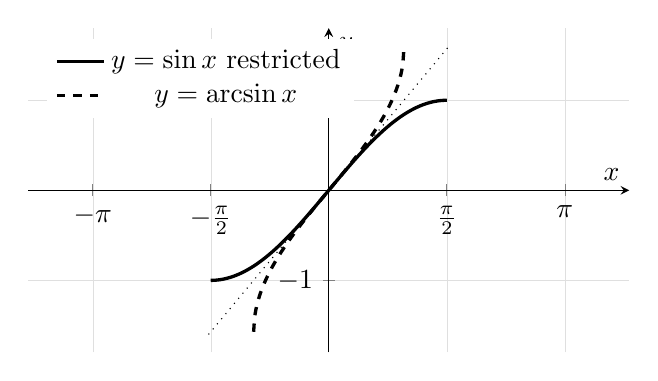
\begin{tikzpicture}
\begin{axis}[
    width=0.76\textwidth,
    height=0.47\textwidth,
    xmin=-4, xmax=4,
    ymin=-1.8, ymax=1.8,
    axis lines=middle,
    xlabel={\(x\)},
    ylabel={\(y\)},
    xtick={-3.1416,-1.5708,0,1.5708,3.1416},
    xticklabels={\(-\pi\),\(-\frac{\pi}{2}\),\(0\),\(\frac{\pi}{2}\),\(\pi\)},
    ytick={-1,0,1},
    grid=both,
    grid style={line width=.1pt, draw=gray!25},
    legend style={draw=none, at={(0.03,0.97)}, anchor=north west}
]
\addplot[very thick, domain=-1.5708:1.5708, samples=150] {sin(deg(x))};
\addlegendentry{\(y=\sin x\) restricted}
\addplot[very thick, dashed, domain=-1:1, samples=150] {rad(asin(x))};
\addlegendentry{\(y=\arcsin x\)}
\addplot[dotted, domain=-1.6:1.6, samples=2] {x};
\end{axis}
\end{tikzpicture}
\caption{The inverse sine reverses the restricted sine function on \([-\pi/2,\pi/2]\).}
\label{fig:appendix-arcsin-graph}
\end{figure}

\paragraph{Example.}
Evaluate

\[
\arccos\left(-\frac12\right).
\]

We need the angle \(y\) in

\[
[0,\pi]
\]

such that

\[
\cos y=-\frac12.
\]

That angle is

\[
\frac{2\pi}{3}.
\]

Therefore

\[
\boxed{
\arccos\left(-\frac12\right)=\frac{2\pi}{3}.
}
\]

\paragraph{Example.}
Evaluate

\[
\arctan(-1).
\]

We need the angle \(y\) in

\[
\left(-\frac{\pi}{2},\frac{\pi}{2}\right)
\]

such that

\[
\tan y=-1.
\]

That angle is

\[
-\frac{\pi}{4}.
\]

So

\[
\boxed{
\arctan(-1)=-\frac{\pi}{4}.
}
\]

\begin{quote}
\textbf{Notation warning.}
The notation

\[
\sin^{-1}x
\]

usually means

\[
\arcsin x,
\]

not

\[
\frac1{\sin x}.
\]

To avoid confusion, this book uses \(\arcsin x\), \(\arccos x\), and \(\arctan x\).
\end{quote}

\subsection{Compositions with inverse trigonometric functions}
\label{appsubsec:compositions-inverse-trig}

The inverse identities work in two directions, but with domains and ranges attached.

For \(-1\le x\le1\),

\[
\boxed{
\sin(\arcsin x)=x.
}
\]

For every \(y\) in

\[
\left[-\frac{\pi}{2},\frac{\pi}{2}\right],
\]

\[
\boxed{
\arcsin(\sin y)=y.
}
\]

The second identity is not true for every real \(y\).  For example,

\[
\arcsin(\sin \pi)=\arcsin(0)=0,
\]

not \(\pi\).

The inverse returns the angle in its chosen range.

\paragraph{Example.}
Simplify

\[
\cos(\arcsin x),
\qquad -1\le x\le1.
\]

Let

\[
\theta=\arcsin x.
\]

Then

\[
\sin\theta=x
\]

and

\[
-\frac{\pi}{2}\le \theta\le \frac{\pi}{2}.
\]

On this interval,

\[
\cos\theta\ge0.
\]

Using

\[
\sin^2\theta+\cos^2\theta=1,
\]

we get

\[
x^2+\cos^2\theta=1.
\]

Thus

\[
\cos^2\theta=1-x^2.
\]

Since \(\cos\theta\ge0\),

\[
\cos\theta=\sqrt{1-x^2}.
\]

Therefore

\[
\boxed{
\cos(\arcsin x)=\sqrt{1-x^2}.
}
\]

The positive square root is not optional.  It comes from the chosen range of arcsine.

\paragraph{Example.}
Simplify

\[
\sin(\arctan x).
\]

Let

\[
\theta=\arctan x.
\]

Then

\[
\tan\theta=x=\frac{x}{1}.
\]

Use a right triangle with opposite side \(x\), adjacent side \(1\), and hypotenuse

\[
\sqrt{x^2+1}.
\]

Since \(\arctan x\) lies in

\[
\left(-\frac{\pi}{2},\frac{\pi}{2}\right),
\]

the adjacent side is positive, and this triangle represents the angle correctly.

Thus

\[
\sin\theta=\frac{x}{\sqrt{x^2+1}}.
\]

Therefore

\[
\boxed{
\sin(\arctan x)=\frac{x}{\sqrt{x^2+1}}.
}
\]

These triangle translations appear often in integration, especially in trigonometric
substitution.

\section{Trigonometric equations}
\label{appsec:trigonometric-equations}

A trigonometric equation usually has many solutions because trigonometric functions
repeat.

Solving one means doing two things:

\[
\text{find the angles on one full cycle}
\]

and then

\[
\text{add the period to describe all repetitions.}
\]

\subsection{Solving by the unit circle}
\label{appsubsec:solving-by-unit-circle}

Start with a simple equation:

\[
\sin x=\frac12.
\]

On one full cycle,

\[
0\le x<2\pi,
\]

the unit circle shows two solutions:

\[
x=\frac{\pi}{6}
\qquad\text{and}\qquad
x=\frac{5\pi}{6}.
\]

Since sine has period \(2\pi\), all solutions are

\[
\boxed{
x=\frac{\pi}{6}+2\pi k
\quad\text{or}\quad
x=\frac{5\pi}{6}+2\pi k,
\qquad k\in\mathbb Z.
}
\]

The integer \(k\) means any whole number:

\[
\ldots,-2,-1,0,1,2,\ldots.
\]

\paragraph{Example.}
Solve

\[
\cos x=-\frac{\sqrt2}{2}
\]

on

\[
0\le x<2\pi.
\]

Cosine is negative in Quadrants II and III.  The reference angle is

\[
\frac{\pi}{4}.
\]

Thus the solutions on one full cycle are

\[
\boxed{
x=\frac{3\pi}{4},\quad \frac{5\pi}{4}.
}
\]

If the problem asks for all real solutions, then

\[
\boxed{
x=\frac{3\pi}{4}+2\pi k
\quad\text{or}\quad
x=\frac{5\pi}{4}+2\pi k,
\qquad k\in\mathbb Z.
}
\]

\paragraph{Example.}
Solve

\[
\tan x=\sqrt3
\]

for all real \(x\).

Tangent has period \(\pi\).  One solution is

\[
x=\frac{\pi}{3}.
\]

Therefore all solutions are

\[
\boxed{
x=\frac{\pi}{3}+\pi k,
\qquad k\in\mathbb Z.
}
\]

\subsection{Solving after using identities}
\label{appsubsec:solving-after-identities}

Many trigonometric equations require an identity before the unit circle can finish the
problem.

\paragraph{Example.}
Solve

\[
2\sin^2 x-\sin x=0
\]

on

\[
0\le x<2\pi.
\]

Factor:

\[
\sin x(2\sin x-1)=0.
\]

So

\[
\sin x=0
\]

or

\[
2\sin x-1=0.
\]

The first equation gives

\[
x=0,\ \pi.
\]

The second equation gives

\[
\sin x=\frac12,
\]

so

\[
x=\frac{\pi}{6},\ \frac{5\pi}{6}.
\]

Therefore the solutions are

\[
\boxed{
x=0,\ \frac{\pi}{6},\ \frac{5\pi}{6},\ \pi.
}
\]

The interval \(0\le x<2\pi\) does not include \(2\pi\), so \(2\pi\) is not listed.

\paragraph{Example.}
Solve

\[
\cos(2x)=\frac12
\]

on

\[
0\le x<2\pi.
\]

First solve for the angle \(2x\).  Since \(x\) runs from \(0\) to \(2\pi\), the angle \(2x\)
runs from \(0\) to \(4\pi\).

Cosine equals \(\frac12\) at

\[
\frac{\pi}{3}
\quad\text{and}\quad
\frac{5\pi}{3}
\]

on the first full cycle, and then repeats after \(2\pi\).  In the interval \(0\le 2x<4\pi\),
we have

\[
2x=\frac{\pi}{3},\ \frac{5\pi}{3},\ \frac{7\pi}{3},\ \frac{11\pi}{3}.
\]

Divide by \(2\):

\[
\boxed{
x=\frac{\pi}{6},\ \frac{5\pi}{6},\ \frac{7\pi}{6},\ \frac{11\pi}{6}.
}
\]

\subsection{Avoiding lost or extra solutions}
\label{appsubsec:trig-equation-warnings}

Trigonometric equations invite two common mistakes.

First, dividing by a trigonometric expression can lose solutions.

Second, squaring both sides can introduce extra solutions.

\paragraph{Example: division can lose solutions.}
Solve

\[
\sin x\cos x=\cos x
\]

on

\[
0\le x<2\pi.
\]

Do not divide by \(\cos x\).  Instead, move all terms to one side:

\[
\sin x\cos x-\cos x=0.
\]

Factor:

\[
\cos x(\sin x-1)=0.
\]

So

\[
\cos x=0
\]

or

\[
\sin x=1.
\]

On \(0\le x<2\pi\),

\[
\cos x=0
\]

at

\[
x=\frac{\pi}{2},\ \frac{3\pi}{2}.
\]

Also,

\[
\sin x=1
\]

at

\[
x=\frac{\pi}{2}.
\]

So the solutions are

\[
\boxed{
x=\frac{\pi}{2},\ \frac{3\pi}{2}.
}
\]

If we had divided by \(\cos x\), we would have lost both cases where \(\cos x=0\).

\paragraph{Example: squaring can add solutions.}
Solve

\[
\sin x=\cos x
\]

on

\[
0\le x<2\pi.
\]

A direct method is to move to tangent.  If

\[
\sin x=\cos x,
\]

then \(\cos x\neq0\), because if \(\cos x=0\), then \(\sin x=\pm1\), not \(0\).
So we may divide by \(\cos x\):

\[
\tan x=1.
\]

Thus

\[
x=\frac{\pi}{4}+\pi k.
\]

On \(0\le x<2\pi\), the solutions are

\[
\boxed{
x=\frac{\pi}{4},\ \frac{5\pi}{4}.
}
\]

If instead we squared both sides, we would get

\[
\sin^2 x=\cos^2 x.
\]

That equation has four solutions on \(0\le x<2\pi\):

\[
\frac{\pi}{4},\ \frac{3\pi}{4},\ \frac{5\pi}{4},\ \frac{7\pi}{4}.
\]

But

\[
\sin x=\cos x
\]

is false at

\[
\frac{3\pi}{4}
\qquad\text{and}\qquad
\frac{7\pi}{4}.
\]

Squaring erased signs.  Always check solutions after squaring.

\section{Practice problems}
\label{appsec:trig-practice-problems}

\subsection*{Unit circle definitions}

\begin{enumerate}
\item Convert \(120^\circ\) to radians.

\item Convert \(\frac{11\pi}{6}\) radians to degrees.

\item A circle has radius \(5\).  Find the arc length cut off by an angle of
\(\frac{3\pi}{4}\) radians.

\item A sector has radius \(4\) and central angle \(\frac{\pi}{3}\).  Find its area.
Use
\[
A=\frac12 r^2\theta
\]
for \(\theta\) in radians.

\item Find \(\sin\theta\), \(\cos\theta\), and \(\tan\theta\) for
\[
\theta=\frac{7\pi}{6}.
\]

\item Find \(\sin\theta\), \(\cos\theta\), and \(\tan\theta\) for
\[
\theta=\frac{3\pi}{4}.
\]
\end{enumerate}

\subsection*{Basic identities}

\begin{enumerate}
\item If
\[
\cos\theta=-\frac35
\]
and \(\theta\) is in Quadrant III, find \(\sin\theta\) and \(\tan\theta\).

\item Simplify:
\[
1-\sin^2 x.
\]

\item Simplify:
\[
\frac{1-\cos^2 x}{\sin x},
\qquad \sin x\neq0.
\]

\item Simplify:
\[
\sec^2 x-\tan^2 x.
\]

\item Verify the identity:
\[
(1-\cos x)(1+\cos x)=\sin^2 x.
\]

\item Simplify:
\[
\sin(-x)+\cos(-x).
\]
\end{enumerate}

\subsection*{Addition formulas}

\begin{enumerate}
\item Simplify:
\[
\sin\left(x+\frac{\pi}{2}\right).
\]

\item Simplify:
\[
\cos(x-\pi).
\]

\item Find the exact value:
\[
\cos\left(\frac{5\pi}{12}\right).
\]

\item Rewrite without powers:
\[
\cos^2 x.
\]

\item Rewrite as a sum:
\[
\sin(5x)\cos(2x).
\]

\item Rewrite as a sum:
\[
\cos(4x)\cos(x).
\]
\end{enumerate}

\subsection*{Inverse trigonometric functions}

\begin{enumerate}
\item Evaluate:
\[
\arcsin\left(-\frac12\right).
\]

\item Evaluate:
\[
\arccos\left(\frac{\sqrt2}{2}\right).
\]

\item Evaluate:
\[
\arctan(\sqrt3).
\]

\item Simplify:
\[
\sin(\arccos x),
\qquad -1\le x\le1.
\]

\item Simplify:
\[
\cos(\arctan 2).
\]

\item Simplify:
\[
\tan\left(\arcsin\frac35\right).
\]
\end{enumerate}

\subsection*{Trigonometric equations}

\begin{enumerate}
\item Solve on \(0\le x<2\pi\):
\[
\sin x=\frac12.
\]

\item Solve on \(0\le x<2\pi\):
\[
\cos x=-\frac{\sqrt3}{2}.
\]

\item Solve on \(0\le x<2\pi\):
\[
\tan x=-1.
\]

\item Solve on \(0\le x<2\pi\):
\[
2\sin^2 x-\sin x=0.
\]

\item Solve on \(0\le x<2\pi\):
\[
\cos(2x)=-\frac12.
\]

\item Solve for all real \(x\):
\[
\sec x=2.
\]

\item Solve for all real \(x\):
\[
\sin x=\cos x.
\]
\end{enumerate}

\section*{Answers to Appendix C practice problems}
\label{ans:appendix-c-practice}

\subsection*{Unit circle definitions}

\begin{enumerate}
\item
\[
120^\circ=120\cdot\frac{\pi}{180}=\frac{2\pi}{3}.
\]

\item
\[
\frac{11\pi}{6}\cdot\frac{180}{\pi}=330^\circ.
\]

\item
\[
s=r\theta=5\cdot\frac{3\pi}{4}=\frac{15\pi}{4}.
\]

\item
\[
A=\frac12 r^2\theta
=
\frac12(4^2)\frac{\pi}{3}
=
\frac{8\pi}{3}.
\]

\item
The angle \(\frac{7\pi}{6}\) is in Quadrant III with reference angle \(\frac{\pi}{6}\).
Thus
\[
\sin\frac{7\pi}{6}=-\frac12,
\qquad
\cos\frac{7\pi}{6}=-\frac{\sqrt3}{2},
\qquad
\tan\frac{7\pi}{6}=\frac{\sqrt3}{3}.
\]

\item
The angle \(\frac{3\pi}{4}\) is in Quadrant II with reference angle \(\frac{\pi}{4}\).
Thus
\[
\sin\frac{3\pi}{4}=\frac{\sqrt2}{2},
\qquad
\cos\frac{3\pi}{4}=-\frac{\sqrt2}{2},
\qquad
\tan\frac{3\pi}{4}=-1.
\]
\end{enumerate}

\subsection*{Basic identities}

\begin{enumerate}
\item
Since
\[
\sin^2\theta+\cos^2\theta=1,
\]
we get
\[
\sin^2\theta=1-\frac{9}{25}=\frac{16}{25}.
\]
In Quadrant III, sine is negative, so
\[
\sin\theta=-\frac45.
\]
Then
\[
\tan\theta=\frac{\sin\theta}{\cos\theta}
=
\frac{-4/5}{-3/5}
=
\frac43.
\]

\item
\[
1-\sin^2 x=\cos^2 x.
\]

\item
\[
\frac{1-\cos^2 x}{\sin x}
=
\frac{\sin^2 x}{\sin x}
=
\sin x,
\qquad \sin x\neq0.
\]

\item
\[
\sec^2 x-\tan^2 x=1.
\]

\item
\[
(1-\cos x)(1+\cos x)=1-\cos^2 x=\sin^2 x.
\]

\item
\[
\sin(-x)+\cos(-x)=-\sin x+\cos x.
\]
\end{enumerate}

\subsection*{Addition formulas}

\begin{enumerate}
\item
\[
\sin\left(x+\frac{\pi}{2}\right)
=
\sin x\cos\frac{\pi}{2}
+
\cos x\sin\frac{\pi}{2}
=
\cos x.
\]

\item
\[
\cos(x-\pi)
=
\cos x\cos\pi+\sin x\sin\pi
=
-\cos x.
\]

\item
\[
\frac{5\pi}{12}=\frac{\pi}{4}+\frac{\pi}{6}.
\]
Thus
\[
\cos\left(\frac{5\pi}{12}\right)
=
\cos\frac{\pi}{4}\cos\frac{\pi}{6}
-
\sin\frac{\pi}{4}\sin\frac{\pi}{6}.
\]
So
\[
\cos\left(\frac{5\pi}{12}\right)
=
\frac{\sqrt2}{2}\cdot\frac{\sqrt3}{2}
-
\frac{\sqrt2}{2}\cdot\frac12
=
\frac{\sqrt6-\sqrt2}{4}.
\]

\item
\[
\cos^2 x=\frac{1+\cos(2x)}{2}.
\]

\item
\[
\sin(5x)\cos(2x)
=
\frac12\bigl(\sin(7x)+\sin(3x)\bigr).
\]

\item
\[
\cos(4x)\cos x
=
\frac12\bigl(\cos(5x)+\cos(3x)\bigr).
\]
\end{enumerate}

\subsection*{Inverse trigonometric functions}

\begin{enumerate}
\item
\[
\arcsin\left(-\frac12\right)=-\frac{\pi}{6}.
\]

\item
\[
\arccos\left(\frac{\sqrt2}{2}\right)=\frac{\pi}{4}.
\]

\item
\[
\arctan(\sqrt3)=\frac{\pi}{3}.
\]

\item
Let
\[
\theta=\arccos x.
\]
Then \(\cos\theta=x\) and \(0\le\theta\le\pi\).  On this interval, \(\sin\theta\ge0\).
Thus
\[
\sin(\arccos x)=\sqrt{1-x^2}.
\]

\item
Let
\[
\theta=\arctan 2.
\]
Then \(\tan\theta=2=\frac{2}{1}\).  The hypotenuse is \(\sqrt5\), so
\[
\cos(\arctan 2)=\frac1{\sqrt5}.
\]

\item
Let
\[
\theta=\arcsin\frac35.
\]
Then \(\sin\theta=\frac35\).  Since \(\theta\in[-\pi/2,\pi/2]\), the cosine is
nonnegative:
\[
\cos\theta=\frac45.
\]
Therefore
\[
\tan\left(\arcsin\frac35\right)
=
\frac{3/5}{4/5}
=
\frac34.
\]
\end{enumerate}

\subsection*{Trigonometric equations}

\begin{enumerate}
\item
\[
\sin x=\frac12
\]
on \(0\le x<2\pi\) gives
\[
\boxed{
x=\frac{\pi}{6},\ \frac{5\pi}{6}.
}
\]

\item
\[
\cos x=-\frac{\sqrt3}{2}
\]
on \(0\le x<2\pi\) gives
\[
\boxed{
x=\frac{5\pi}{6},\ \frac{7\pi}{6}.
}
\]

\item
\[
\tan x=-1
\]
on \(0\le x<2\pi\) gives
\[
\boxed{
x=\frac{3\pi}{4},\ \frac{7\pi}{4}.
}
\]

\item
\[
2\sin^2 x-\sin x=0
\]
factors as
\[
\sin x(2\sin x-1)=0.
\]
So
\[
\sin x=0
\quad\text{or}\quad
\sin x=\frac12.
\]
On \(0\le x<2\pi\),
\[
\boxed{
x=0,\ \frac{\pi}{6},\ \frac{5\pi}{6},\ \pi.
}
\]

\item
For
\[
\cos(2x)=-\frac12,
\]
with \(0\le x<2\pi\), we have \(0\le2x<4\pi\).  Cosine equals \(-1/2\) at
\[
2x=\frac{2\pi}{3},\ \frac{4\pi}{3},\ \frac{8\pi}{3},\ \frac{10\pi}{3}.
\]
Divide by \(2\):
\[
\boxed{
x=\frac{\pi}{3},\ \frac{2\pi}{3},\ \frac{4\pi}{3},\ \frac{5\pi}{3}.
}
\]

\item
\[
\sec x=2
\]
means
\[
\cos x=\frac12.
\]
Thus
\[
\boxed{
x=\frac{\pi}{3}+2\pi k
\quad\text{or}\quad
x=\frac{5\pi}{3}+2\pi k,
\qquad k\in\mathbb Z.
}
\]

\item
\[
\sin x=\cos x
\]
gives
\[
\tan x=1.
\]
Thus
\[
\boxed{
x=\frac{\pi}{4}+\pi k,
\qquad k\in\mathbb Z.
}
\]
\end{enumerate}